\documentclass[12pt, a4paper, tocpage=plain]{abnt} % Fonte tamanho 12, papel A4, páginas do sumário sem o p.<número da página>

\usepackage[utf8]{inputenc} % Dá suporte para caracteres especiais como acentos e cedilha
\usepackage[brazil]{babel} % Gera datas e nomes em português com estilo brasileiro
\usepackage{hyperref} % Permite a criação de hyperlink no documento, como os links usados na referência
\usepackage[alf]{abntcite} % Define o estilo de referência bibliográfica
\usepackage{graphicx} % Permite a utilização de imagens no documento
\usepackage[small]{caption} % Define as legendas das figuras com fontes menores do que o texto
\usepackage{pslatex} % Define que o formato da letra será Times New Roman
\usepackage{epigraph} % Permite a criação de epígrafes 
\usepackage{setspace} % Permite a definição de espaçamento entre linhas
\usepackage[top=3cm, left=3cm, right=2cm, bottom=2cm]{geometry} % Define as margens da folha
\usepackage{appendix}

\setcounter{secnumdepth}{3} % Até três subsubsections numeradas
\setcounter{tocdepth}{3} % Até trẽs subsubsections numeradas

\setlength{\parindent}{1.25cm} % Define o recuo da primeira linha dos parágrafos para 1.25 cm

\renewcommand{\ABNTchapterfont}{\bfseries} % Define a fonte do \chapter
\renewcommand{\ABNTchaptersize}{\large} % Define o tamanho da fonte do \chapter
\renewcommand{\ABNTsectionfontsize}{\large} % Define o tamanho da fonte da \section
\renewcommand{\ABNTsubsectionfontsize}{\large} % Define o tamanho da fonte do \subsection
\renewcommand{\ABNTsubsubsectionfontsize}{\large} % Define o tamanho da fonte do \subsubsection
\renewcommand{\ABNTbibliographyname}{REFERÊNCIAS BIBLIOGRÁFICAS} % Modifica o título gerado pelo \bibliographys

\begin{document} % Começo do TCC
\begin{titlepage}
 \begin{figure}[ht]
 \centering
 \scalebox{0.35}{
\includegraphics{figuras/logo}}
 \end{figure}
 \begin{center}
   {\large CURSO DE TECNOLOGIA EM DESENVOLVIMENTO DE SOFTWARE} \\ [5.5cm]
   {\large JOÃO FELIPE ROQUE MORAES} \\ [4cm]
   {\large APRESENTAÇÃO, ESTUDO E PROPOSTA DE USO DO \textit{HARDWARE RASPBERRY PI} EM PEQUENAS EMPRESAS } \\
   \vfill
   {\large Campos dos Goytacazes/RJ} \\
   {\large 2013}
 \end{center}
\end{titlepage}
 % Cria a capa
\begin{titlepage}
 \begin{figure}[ht]
 \centering
 \scalebox{0.35}{
\includegraphics{figuras/logo}}
 \end{figure}
 \begin{center}
   {\large CURSO DE TECNOLOGIA EM DESENVOLVIMENTO DE SOFTWARE} \\ [3.5cm]
   {\large JOÃO FELIPE ROQUE MORAES} \\ [4cm]
   {\large APRESENTAÇÃO, ESTUDO E PROPOSTA DE USO DO \textit{HARDWARE RASPBERRY PI} EM PEQUENAS EMPRESAS } \\ [2cm]
   \hspace{.45\textwidth} % posicionando a minipage
   \begin{minipage}{0.5\textwidth}
   \begin{espacosimples}
        Trabalho de conclusão de curso apresentado ao Instituto Federal Fluminense como requisito parcial para conclusão do Curso de Tecnologia em Desenvolvimento de Software.\\[1.5cm]
        Orientador: Prof. Fernando Carvalho
    \end{espacosimples}
    \end{minipage}
   \vfill
   {\large Campos dos Goytacazes/RJ} \\
   {\large 2013}
 \end{center}
\end{titlepage}
 % Cria a folha de rosto
\begin{folhadeaprovacao}
    \setlength{\ABNTsignthickness}{0.4pt}
    \setlength{\ABNTsignwidth}{15cm}
    \setlength{\ABNTsignskip}{0.9cm}
    \begin{center}
        {\large JOÃO FELIPE ROQUE MORAES} \\ [4cm]
        {\large APRESENTAÇÃO, ESTUDO E PROPOSTA DE USO DO \textit{HARDWARE RASPBERRY PI} EM PEQUENAS EMPRESAS } \\ [2cm]
        \hspace{.45\textwidth} % posicionando a minipage
        \begin{minipage}{0.5\textwidth}
        \begin{espacosimples}
        Trabalho de conclusão de curso apresentado ao Instituto Federal Fluminense como requisito parcial para conclusão do Curso de Tecnologia em Desenvolvimento de Software.\\\\
        \end{espacosimples}
        \end{minipage}
    \end{center}
    Aprovada em 04 de outubro de 2013 \\\\
    Banca avaliadora:
    \assinatura{Prof. Fernando Carvalho (Orientador) \\ Especialista em Produção e Sistemas / IFF Campus Campos \\ Instituto Federal de Educação, Ciência e Tecnologia Fluminense / Campus Bom Jesus}
    \assinatura{Prof. Rogério Atem Carvalho \\ Doutor em Ciências de Engenharia / IFF Campus Campos \\ Instituto Federal de Educação, Ciência e Tecnologia Fluminense / Campus Campos Centro}
    \assinatura{Prof. Fábio Duncan de Souza \\ Mestre em Pesquisa Operacional e Inteligência Computacional / UCAM Campos \\ Instituto Federal de Educação, Ciência e Tecnologia Fluminense / Campus Campos Centro}
\end{folhadeaprovacao} % Cria a folha de aprovação
\null
\vfill

{\normalsize \it \hfill À minha família, \vspace*{4pt}

\hfill com amor\dots}
  % Cria a folha de dedicatória
\begin{center}
\textbf{AGRADECIMENTOS}
\end{center}

Quero agradecer primeiramente àquele que é o meu melhor amigo, que sempre está comigo e que nunca irá abandonar-me, Jesus Cristo. Agradeço por ter me abençoado no aprendizado ao longo da vida, o que me permitiu não somente a oportunidade de passar no processo seletivo para esta instiuição, como também, no dia de hoje, a me formar na minha graduação. À Ele seja a glória.

Agradeço à minha família, base sólida sobre a qual eu me desenvolvi. Aos meus pais e meu irmão, obrigado por me fornecerem ânimo durante a caminhada desta graduação.

Como não mencionar o Núcleo de Pesquisa em Sistemas de Informação (NSI) pela rica oportunidade de logo no primeiro período de curso já poder praticar e aprender programação.

Agradeço à minha namorada Juliana pelas orações e palavras de apoio, e a todos os meus amigos e colegas que contribuíram para que esse trabalho fosse concluído. 

Por último, mas não com menos importância, gostaria de agradecer ao meu orientador Fernando Carvalho pelas dicas, paciência demostrada a mim. % Cria a folha de agradecimentos
\null % o \vfill só funciona com o \null
\vfill
\epigraph{Pois, que adianta ao homem ganhar o mundo inteiro e perder a sua alma?}{Jesus Cristo}
 % Cria a epígrafe (onde se coloca um pensamento)
\begin{center}
\textbf{RESUMO}
\end{center}
\singlespacing

\noindent Este trabalho de conclusão de curso apresenta o \textit{hardware Raspberry PI} e investiga a possibilidade do mesmo ser uma alternativa de baixo custo para a implantação de computadores e sistemas em pequenas empresas associado a utilização de sistemas \textit{web}. Desta forma, para avaliar o produto em um empreendimento no mundo real, o dispositivo e sua implementação foram avaliados, e foi desenhado um estudo de caso da sua implantação, o que viabilizou conclusões sobre a utilização da nova tecnologia em pequenas organizações.\\

\noindent PALAVRAS-CHAVE: Desenvolvimento de \textit{Software}, \textit{Raspberry Pi}, Pequenas Empresas
 % Resumo do trabalho
\begin{center}
\textbf{ABSTRACT}
\end{center}

\singlespacing

\noindent  \\

\noindent KEYWORDS: 
 % Resumo em língua estrangeira
\renewcommand{\listfigurename}{LISTA DE FIGURAS} % Modifica o nome da lista de figuras
\listoffigures % Gera o índice de figuras
\renewcommand{\contentsname}{SUMÁRIO} % Modifica o nome do sumário
\tableofcontents % Gera o sumário
\onehalfspacing % Define o espaçamento de 1.5cm entre linhas
\chapter{INTRODUÇÃO}

A Tecnologia da Informação (TI) pode ser definida como o conjunto de todas as atividades e soluções fornecidas por recursos de computação que visam permitir a produção, armazenamento, transmissão, acesso e o uso das informações \cite{WIKIPEDIA}.

É sabido que para empresas, o tratamento das suas informações são uma fonte de estratégias para lucrar ou conter desperdícios. Segundo \citeonline{LAURINDO}, a TI evoluiu de uma orientação tradicional de suporte administrativo para um papel estratégico dentro da organização . Dessa forma, fica evidente que na sociedade da informação, as modernas TI têm influenciado decisivamente as organizações, tanto as grandes quanto as pequenas empresas \cite{CRISTINA}.

Nas micro e pequenas empresas (MPE), a TI assume ainda um papel mais importante, que está relacionado ao tempo de vida no mercado. Nesse contexto, os sistemas de informação, através das várias tecnologias disponíveis, podem contribuir para a sobrevivência e desenvolvimento das MPE, constituindo-se em ferramenta estratégica para enfrentar e superar desafios \cite{VALDIR}.

A infraestrutura de TI entretanto é cara, sendo necessário viabilizar recursos com custos mais compatíveis com pequenas organizações.

A partir de 2006 tornou-se disponível o hardware raspberry pi,  que pode ser útil e apresentar um custo benefício interessante para empresas de pequeno porte.

O objetivo deste trabalho é estudar e apresentar as características deste dispositivo, avaliar seu potencial de uso, bem como exemplificar seu uso para ambientes comerciais. Desta forma será possível iniciar a avaliação do hardware em ambiente acadêmico e analisar critérios como custo, desempenho, robustez, escalabilidade e operabilidade.

% \section{Estrutura do trabalho}

% Este trabalho se divide em 5 capítulos e está estruturado da seguinte maneira:

% No capítulo 2 é feita uma fundamentação de conceitos e técnicas necessárias para o entendimento deste trabalho. METODOLOGIA

% No capítulo 3 é feita uma descrição da Integração Contínua, seus componentes, suas práticas e suas vantagens. REFERENCIAL TEÓRICO

% Já no capítulo 4, é apresentado um estudo de caso, em que os autores deste trabalho são responsáveis por implantar um ambiente de Integração Contínua, em um projeto real de desenvolvimento de software. CARACTERÌSTICAS TÈCNICAS

% E por fim, o capítulo 5 apresenta os resultados obtidos com o estudo de caso bem como os trabalhos futuros a serem desenvolvidos no processo da Integração Contínua implantado no projeto. CONFIGURAÇÕES POSSIVEIS

% ESTUDO DE CASO

% RESULTADOS OBTIDOS


 % Cria o capítulo 1
\chapter{METODOLOGIA}



Inicialmente o professor orientador deste trabalho realizou a compra do equipamento, e em seguida buscou-se realizar testes que demonstrassem que o \textit{Raspberry Pi} seria um bom tema a ser discutido nesta monografia. Os testes foram: ligar o equipamento, analisar as funcionalidades apresentadas pelo sistema operacional e realizar tarefas simples, como acessar a internet, usar a calculadora e abrir um arquivo de extensão .pdf. Quando executados, todos os testes citados anteriormente retornaram seus resultados com tempo de resposta normal, sem apresentar lentidão.

Desta forma, iniciou-se uma revisão bibliográfica para a pesquisa e obtenção de informações sobre o \textit{Raspberry Pi} que viabilizassem a escrita de um referencial teórico, sessão responsável por apresentar uma sequência de assuntos com a finalidade de fornecer embasamento conceitual para o entendimento deste trabalho.

Pautando-se nos resultados dos testes comentados no primeiro parágrafo e na análise do referencial teórico, foi planejado um estudo de caso que avaliasse a utilização do \textit{Raspberry Pi} num ambiente de produção. Tal avaliação foi realizada na Assessoria de Suporte da Gerência de Informação da Universidade Estadual do Norte Fluminense Darcy Ribeiro, onde funcionários trabalham diariamente utilizando um sistema \textit{web} para gerenciar as demandas na área de tecnologia da informação.

Após o uso do equipamento pelos integrantes do setor, foi fornecido um questionário, que visa quantificar a satisfação qualitativamente, e com isso avaliar a adequação para o caso específico. O resultados do questionário foram analisados e discutidos para produzir as conclusões do trabalho. % Cria o capítulo 2 
\chapter{REFERENCIAL TEÓRICO}

No mundo atual podemos encontrar diferentes classificações de sistemas computacionais. Existem os de grande porte, conhecidos como \textit{mainframes}, os de médio porte, como os servidores e \textit{workstations}, e os de pequeno porte, que podem ser divididos em duas categorias: os de mesa (\textit{desktops}) e os portáteis (\textit{notebooks}).

Os tipos de computadores citados no parágrafo anterior são utilizados a partir da necessidade de cada usuário. \textit{Mainframes}, por exemplo, são usados para processar um grande volume de informações, enquanto que \textit{desktops} ou \textit{notebooks} atendem à demandas que exigem um menor poder de processamento.

Desta forma, existindo diferenças nos objetivos de uso de cada equipamento, e também uma disparidade considerável entre os custos dos mesmos, os microcomputadores estão entre os mais utilizados nos dias atuais, pois têm um custo acessível e atendem às necessidades dos usuários comuns de forma eficiente. Até empresas poderiam conter gastos, sem deixar a desejar na qualidade do serviço prestado, se substituíssem computadores de grande porte por outros de pequeno porte. Essa iniciativa contemplaria o cenário de uma técnica chamada \textit{downsizing}.

\section{\textit{Downsizing}}

Na área da informática o termo \textit{downsizing} define uma situação onde sistemas originalmente hospedados em um computador de grande porte (\textit{mainframe}) são adaptados para computadores de menor porte (microcomputadores), e esse processo consiste em função da redução do porte da empresa ou do aumento da capacidade computacional dos computadores de menor custo \cite{WIKIPEDIA3}.

\section{\textit{Thin client}}

Segundo \citeonline{TOM}, \textit{thin clients} são sistemas básicos de informática que trabalham com um servidor para processar aplicações e armazenar dados por meio da virtualização; quase todo o processamento ocorre no servidor, e a maior parte dos programas são instalados e gerenciados virtualmente por um gerente de TI.

\begin{figure}[ht]
    \centering
    \scalebox{0.7}{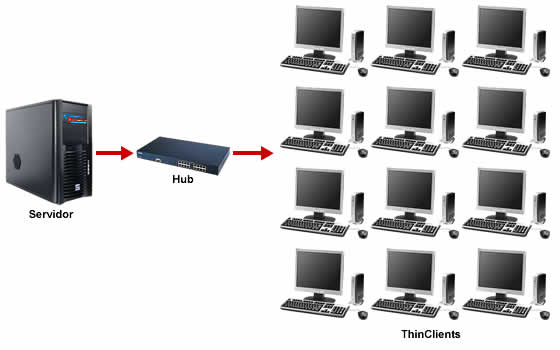
\includegraphics{figuras/rede_thin_clients}}
    \caption{Representação de uma rede de computadores com \textit{thin clients}. Adaptado de \cite{THINCLIENT}}
\end{figure}

Com a implantação de \textit{thin clients} e apenas um computador (\textit{host} ou servidor) é possível gerar várias estações de acesso. A configuração do servidor depende do número de terminais e das necessidades dos usuários da rede. Esta deve ser minuciosamente analisada antes de elaborar e formatar o ambiente utilizado.

Da mesma forma que um \textit{thin client} processa poucos dados, deixando o maior volume do processamento para o servidor, um sistema construído para arquitetura \textit{web} também tem suas funcionaliades executadas pelo servidor que o hospeda, deixando o computador do usuário responsável por apresentar resultados do processamento. Desta forma, mesmo que a estação de trabalho do usuário final tenha recursos limitados, será possível utilizar o sistema normalmente.

No estudo de caso que será efetuado neste trabalho, o \textit{Raspberry Pi} irá respeitar esse modelo de processamento, pois o sistema criado para gerenciar as demandas do setor alvo da pesquisa foi desenvolvido utilizando arquitetura \textit{web}.

\section{Barateamento dos equipamentos de mesa}

Atualmente, sob a ótica financeira, comprar um computador não é mais uma tarefa impossível, mas há alguns anos os preço desses equipamentos eram muito pouco acessíveis. Chega a ser difícil crer que a cerca de 15 anos o valor pago por um computador com configurações totalmente inferiores às dos computadores atuais, era de R\$ 4 mil, aproximadamente \cite{HAMANN}.

Para se entender o por quê dos altíssimos preços desses equipamentos, é preciso atentar-se para o ciclo de vida das tecnologias. Aparelhos que custam muito têm seus valores reduzidos gradativamente até que cheguem aos preços mais populares, então surgem novas tecnologias, fazendo com que a curva dos preços volte a subir e o ciclo se repita. Isso pode ser percebido com televisores e suas diferentes tecnologias: CRT, LCD, Plasma, LED e os novos modelos 3D que ainda estão com preços altíssimos \cite{HAMANN}.

Em se tratando de informática, não é diferente. Os componentes de hardware sempre são lançados com valores altos que, com o passar do tempo, são reduzidos. Um dos fatores que mais contribui para a redução nos preços é a evolução tecnológica, pois quando são lançados novos produtos, é necessário reduzir os valores dos mais antigos para que eles não fiquem presos nas fábricas \cite{HAMANN}. Essa maior acessibilidade provocada pela evolução técnológica pode ser muito útil quando se observa o cenário das pequenas empresas no Brasil.

\section{Realidade de pequenas empresas como maior categoria de empresas no Brasil}

As pequenas e médias empresas (MPEs) são fundamentais para promover o crescimento econômico, criar empregos e renda e melhorar as condições de vida da população. Os indicadores desse segmento empresarial demonstram sua importância na economia, não só no Brasil, mas em todo o mundo \cite{PORTALBRASIL}.

A contribuição das MPEs é reconhecida principalmente na capilaridade que estes negócios propiciam e na absorção de mão de obra, inclusive aquela com maior dificuldade de inserção no mercado, como jovens em busca pelo primeiro emprego e as pessoas com mais de 40 anos. As pequenas empresas também são capazes de dinamizar a economia dos municípios e bairros das grandes metrópoles \cite{PORTALBRASIL}.

“Pequenas empresas são o sustentáculo de uma economia em qualquer lugar do mundo. São elas que agregam valor a produtos e serviços”, afirma o diretor executivo do Centro de Inovação, Empreendedorismo e Tecnologia (Cietec), incubadora de empresas da Universidade de São Paulo (USP), Sérgio Risola. Segundo dados mais recentes do IBGE, as MPEs representam 20\% do Produto Interno Bruto (PIB) brasileiro, são responsáveis por 60\% dos 94 milhões de empregos no país e constituem 99\% dos 6 milhões de estabelecimentos formais existentes no país. A maior parte dos negócios estão localizados na região Sudeste (com quase 3 milhões de empresas) e o setor preferencial é o comércio, seguido de serviços, indústria e construção civil \cite{PORTALBRASIL}.

Desde 2000, a participação das MPEs no total de empreendimentos produtivos brasileiros aumentou bastante. Enquanto a taxa de crescimento anual foi de 4\% para o total de empresas, independente do porte, para as pequenas empresas foi de 6,2\%, e 3,8\% para as micro, entre 2000 e 2008. Nesse mesmo período, as MPEs foram responsáveis por aproximadamente metade dos postos de trabalho formais criados, ou seja, 4,5 milhões de empregos \cite{PORTALBRASIL}.

O faturamento das MPEs também cresceu consideravelmente nos últimos anos. No primeiro semestre de 2010, a receita real registrou aumento de 10,7\% comparado ao mesmo período de 2009. Este indicador aponta que as pequenas empresas superam o ritmo de crescimento da economia brasileira. Essa é a maior taxa de crescimento de faturamento desde que o Sebrae iniciou a pesquisa, em 1998 \cite{PORTALBRASIL}.

\begin{table}[!htpb]
 \centering
    \begin{tabular}{|l|p{5cm}|c|} 
    \hline
        \textbf{As MPEs no Brasil} & \textbf{O que isso representa} \\
    \hline
        20\% do PIB & R\$ 700 bilhões \\
    \hline
        99\% das empresas & R\$ 5,7 milhões de MPEs \\
    \hline
        60\% dos empregos & R\$ 56,4 milhões de empregos \\
    \hline
    \end{tabular}
    \caption{Estatísticas das MPEs no Brasil}
    \label{t_fixa}
\end{table} % Cria o capítulo 3
\chapter{CARACTERÍSTICAS TÉCNICAS DA PLATAFORMA \textit{RASPBERRY PI}}

\textit{Raspberry Pi} é um computador do tamanho de um cartão de  rédito desenvolvido no Reino Unido pela Fundação \textit{Raspberry Pi} com a intenção de estimular o ensino de informática básica nas escolas. Ele se conecta à sua TV e a um teclado, e pode ser usado para muitas das coisas que o seu PC \textit{desktop} faz, como processar textos, planihas e jogos, além de reproduzir vídeo de alta definição. Todo o \textit{hardware} é integrado em uma única placa, e o projeto é baseado em um \textit{system on a chip} (SoC) Broadcom BCM2835, que inclui um processador ARM1176JZF-S de 700 MHz, GPUVideoCore IV, e 512 MB de memória RAM em sua última revisão. O projeto não inclui uma memória não-volátil - como um disco rígido - mas possui uma entrada de cartão SD para armazenamento de dados. A placa é adaptada para rodar sistemas operacionais baseados em Linux \cite{WIKIPEDIA2}.

\subsection{História}

A ideia de criar um computador pequeno e barato para crianças surgiu em 2006, quando Eben Buton e seus colegas da Universidade de Cambridge perceberam que os estudantes de hoje que querem estudar ciência da computação não têm as habilidades que eles tinham na década de 1990. Eles atribuem isso, entre outros fatores, à ascensão do computador pessoal (PC) e dos \textit{consoles} de jogos que substituíram os microcomputadores. Desde que o computador tornou-se importante para todos os membros da família, o ato de deixar os membros mais jovens brincarem ou fazerem experimentos foi sendo cada vez mais desestimulado.

Mas recentemente os processadores usados em telefones celulares e tablets tornaram-se mais baratos e mais poderosos, abrindo caminho para o lançamento do \textit{Raspeberry Pi} no mundo das placas de computadores ultrabaratas e úteis.

\subsection{Viabilidade no mercado brasileiro}

Para se obter um \textit{Raspberry Pi} no Brasil é preciso importá-lo. No site da farnellwark, empresa que realiza serviços de importação e revenda, o valor da placa \textit{Raspberry Pi} - Modelo B é R\$ 176,02. O preço apresentado anteriormente é um somatório do custo real da placa com despesas referentes à importação, sendo que o frete para a entrega do equipamento em sua residência ainda não está incluso. Para se ter uma noção do aumento no valor da compra gerado pela despesas com importação, foi pesquisado o preço em um site que vendesse a mesma placa sem tais custos. No site da adafruit, o preço encontrado foi de \$ 39,95, o equivalente a R\$ 88,61, de acordo com a cotação do dólar às 12h do dia 21 de setembro de 2013, evidenciando assim uma diferença de R\$ 87,49.

\begin{table}[!htpb]
 \centering
    \begin{tabular}{|l|p{3cm}|c|} 
    \hline
        \textbf{Valor} & \textbf{Impostos} & \textbf{Valor Total} \\
    \hline
        R\$ 90,93 & R\$ 87,49 & R\$ 176,02 \\
    \hline
    \end{tabular}
    \caption{Apresentação do valor do \textit{Raspberry Pi} agregado com gastos de importação para o Brasil. O valor total não inclui o frete.}
    \label{t_fixa}
\end{table}

O frete e o tempo de entrega do equipamento em residência varia de acordo com a localidade da mesma. Para uma entrega em Campos dos Goytacazes, o valor do frete cobrado foi de R\$ 32,20 e o tempo de 3 dias úteis.

Em relação a empresas que oferecem suporte à placa no Brasil não foi encontrada nenhuma informação.

\subsection{Comparativo de custos de \textit{hardware} semelhante}

Para apresentar a diferença de custo entre o \textit{Raspberry Pi} e um \textit{hardware} semelhante, mais precisamente um computador \textit{desktop}, foram escolhidas duas empresas para serem alvos da pesquisa de preço. A primeira será a Farnell Newark, empresa já apresentada na seção anterior e que fornecerá o valor do \textit{Raspberry Pi}, e a segunda será a Americamas.com, empresa que informará o preço do PC \textit{desktop} mais barato existente na loja. Em ambas as empresas tal pesquisa de preço foi realizada às 14:18 horas do dia 28 de setembro de 2013.

O valor apresentado pela Farnell Newark para o \textit{Raspberry Pi} foi de R\$ 176,02 mais despesas com frete, enquanto que a loja Americanas.com vende o pc \textit{desktop} mais barato pelo preço de R\$ 719,00.

Ao se analisar os valores apresentados no parágrafo anterior, é preciso entender que a comparação entre os equipamentos não acontece em torno da capacidade de seus componentes, tais como poder de processamento, quantidade de memória RAM, capacidade de disco rígido, e etc, pois se assim fosse o pc \textit{desktop} desbancaria a nova tecnologia que está sendo apresentada. O objetivo do comparativo está em mostrar o bom custo x benefício que o  \textit{Raspberry Pi} pode apresentar.

\subsection{Sistemas computacionais que utilizam o \textit{Raspberry Pi}}

Apesar de os idealizadores do \textit{Raspberry Pi} o terem criado visando uma prática maior da programação entre jovens e crianças, o equipamento tem sido utilizado por pessoas do mundo inteiro a fim de alcançarem outros objetivos. Sendo assim, foram pesquisados projetos que apresentassem exemplos do uso do equipamento em sistemas computacionais, e o resultado a seguir.

Em um artigo escrito por \citeonline{PEDRO}, o \textit{Raspberry Pi} é utilizado como um servidor de \textit{Virtual Private Network} (VPN) ou Rede Privada Virtual. Após demonstrar passo a passo a instalação de alguns pacotes e realizar algumas configurações necessárias, o autor do artigo explica que ao se conectar a uma rede pública e necessitar da garantia que a sua conexão é segura, pode-se fazer uso do \textit{Raspberry Pi} para que as conexões sejam cifradas e que passe por ele.

Segundo \citeonline{ZACH}, é possível fazer do \textit{Raspberry Pi} um servidor web barato para realizar testes ou armazenar arquivos.

Nota-se então que já se encontram exemplos de sistemas computacionais baseados no \textit{Raspberry Pi}, o que multiplica as possíveis utilidades dessa nova tecnologia.

\subsection{Descrição técnica}

\begin{figure}[ht]
    \centering
    \scalebox{0.41}{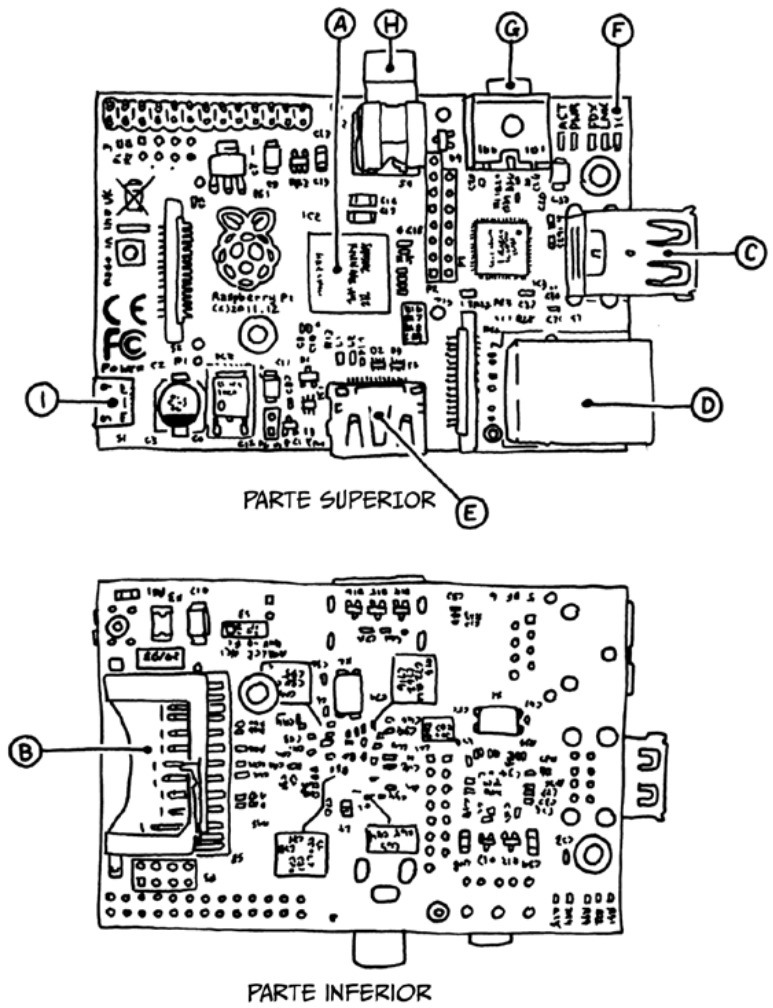
\includegraphics{figuras/superior_inferior}}
    \caption{Ilustração da placa \textit{Raspberry Pi}}
\end{figure}

A Figura 4.1 representa a placa do computador \textit{Raspberry Pi} contendo indicações em diversos componentes, os quais serão melhor especificados a seguir.

\textbf{A. Processador.} No coração do \textit{Raspberry Pi} está o mesmo processador que você encontraria no iPhone 3G e no Kindle 2, assim você pode pensar nas capacidades do \textit{Raspberry Pi} como comparáveis a esses poderosos pequenos aparelhos. Este processador trabalha na frequência de 700 MHz - 32 bits, e foi construído sobre a arquitetura ARM11. Chips ARM apresentam-se em uma variedade de arquiteturas com diferentes núcleos configurados para fornecer diferentes capacidades com preços diferentes. O modelo B tem 512 MB de memória RAM e o modelo A tem 256 MB. (O primeiro lote do modelo B tinha apenas 256 MB de RAM.)
    
\textbf{B. Slot para cartão de memória SD (Secure Digital).} Você perceberá que não há disco rígido no Pi; tudo é armazenado em um cartão de memória SD. Uma razão pela qual você irá desejar, mais cedo ou mais tarde, algum tipo de gabinete (case) de proteção, é que as soldas no soquete SD poderão quebrar se o cartão for acidentalmente dobrado.

\textbf{C. Porta USB.} No modelo B há duas portas USB 2.0, mas apenas uma no modelo A. Algumas das primeiras placas do \textit{Raspberry Pi} foram limitadas quanto à quantidade de corrente que elas poderiam fornecer. Alguns dispositivos USB podem chegar a 500mA. A placa original do Pi suportava 100mA ou quase, mas as revisões mais recentes alcançam até a especificação completa das portas USB 2.0. Provavelmente não é uma boa ideia recarregar seu celular com o \textit{Raspberry Pi}. Você poderá usar um hub com alimentação externa se tiver um periférico que necessite de mais energia.

\textbf{D. Porta Ethernet.} O modelo B tem uma porta Ethernet padrão RJ45. O modelo A não tem, mas pode ser conectado a uma rede com fios por meio de um adaptador de rede Ethernet USB (a porta no modelo B é na verdade um adaptador Ethernet USB embutido). A conectividade Wi-Fi por meio de um adaptador USB externo é outra opção.

\textbf{E. Conector HDMI.} A porta HDMI oferece saída de áudio e vídeo digital. Catorze resoluções de vídeo diferentes são suportadas, e o sinal HDMI, por meio de adaptadores externos, pode ser convertido para DVI (usado por muitos monitores), vídeo composto (sinal de vídeo analógico normalmente transmitido por um conector RCA amarelo), ou SCART (uma norma europeia para conexão de equipamentos audiovisuais).

\textbf{F. LEDs de status.} O Pi tem cinco LEDs indicadores de status que podem ser visualizados na Tabela 4.1 abaixo.

\begin{table}[!htpb]
 \centering
    \begin{tabular}{|l|p{2cm}|l|} 
    \hline
        \textbf{Led} & \textbf{Cor} & \textbf{Descrição} \\
    \hline
        ACT & Verde & Acende quando o cartão SD é acessado \\
    \hline
        PWR & Vermelho & Conectado à alimentação de 3.3V \\
    \hline
        FDX & Verde & On (ligado) se o adptador de rede é full-duplex \\
    \hline
        LNK & Verde & Luz indicando atividade de rede \\
    \hline
        100 & Amarelo & On (ligado) se a conexão de rede for 100Mpbs \\
    \hline
    \end{tabular}
    \caption{LEDs com cindo indicações de status}
    \label{t_fixa}
\end{table}

\textbf{G. Saída de áudio analógico.} É um conector de áudio analógico padrão de 3,5 mm que é destinado a conduzir cargas de alta impedância (como alto-falantes amplificados). Fones de ouvido ou alto-falantes sem alimentação não terão som de qualidade. Parte desse problema tem a ver com o software controlador de áudio, o qual ainda está em desenvolvimento.

\textbf{H. Saída de vídeo composto.} É um conector-padrão tipo RCA que fornece sinais de vídeo composto NTSC ou PAL. Esses formatos de vídeo têm resolução extremamente baixa se comparada com HDMI. Se você tiver um monitor ou um televisor com entrada HDMI, use-o em vez de um televisor com entrada de vídeo composto.

\textbf{I. Entrada de energia.} Uma das primeiras coisas que você perceberá é que não há nenhum interruptor de alimentação no \textit{Raspberry Pi}. Esse conector micro USB é usado para fornecer energia (essa não é uma porta USB adicional, é apenas para alimentação). A porta micro USB foi escolhida porque o conector é barato e fontes de alimentação USB são fáceis de encontrar.

\newpage

\subsection{Periféricos adequados}

Após adquirir-se um pouco de conhecimento sobre os componentes da placa, faz-se necessário saber também sobre os periféricos adequados para utilizar com ela. A imagem abaixo mostra alguns dos quais iremos precisar para utilizar o \textit{Raspberry}. É preciso tomar cuidado, pois existem peças que podem não funcionar corretamente quando instaladas na sua placa.

\begin{figure}[ht]
    \centering
    \scalebox{0.27}{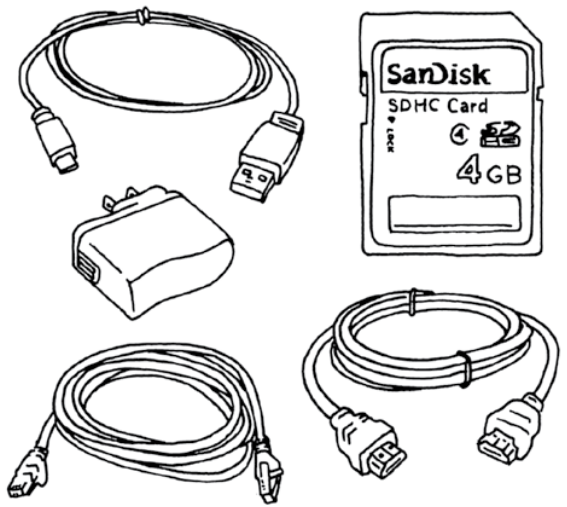
\includegraphics{figuras/perifericos_adequados}}
    \caption{Periféricos básicos: uma fonte de alimentação micro USB, cabos e cartão SD.}
\end{figure}

\textbf{Fonte de alimentação.} Este é o periférico mais importante para ser obtido. Você deve usar um adaptador micro USB que pode fornecer 5V e pelo menos 700mA de corrente (500mA para o modelo A). Um carregador de telefone celular não vai funcionar, mesmo se ele tiver o conector correto. Um carregador de telefone celular típico fornece apenas 400mA de corrente ou menos, mas verifique a classificação indicada na parte de trás. Um \textit{Raspberry Pi} com fonte de alimentação inferior pode parecer funcionar, mas ficará estranho e poderá falhar (travar) de forma imprevisível. Um problema comum causado por insuficiência de corrente descrito pelos usuários do \textit{Raspberry Pi} é que o teclado não funciona corretamente.

\textbf{Cartão SD.} Você vai precisar de pelo menos 4GB, e deve ser um cartão de Classe 4. Estes cartões são capazes de transferir pelo menos 4MB/seg. Algumas das placas anteriores do \textit{Raspberry Pi} apresentaram problemas com cartões de Classe 6 ou superiores, os quais são capazes de velocidades mais rápidas, mas com menos estabilidade. Um cartão micro SD em um adaptador é perfeitamente utilizável também.

\textbf{Cabo HDMI.} Se você está se conectando a um monitor, precisará deste cabo ou um adaptador apropriado para um monitor DVI. Você também pode executar o Pi sem monitor, como descrito posteriormente neste capítulo. Cabos HDMI podem variar muito de preço. Se está instalando um cabo de 90 a 180 cm para o monitor, não há necessidade de gastar mais de US\$ 3 em um cabo HDMI. Se estiver instalando comprimentos maiores, você definitivamente deve pesquisar cabos de maior qualidade e evitar os genéricos mais baratos.

\textbf{Cabo Ethernet.} Visto que atualmente praticamente tudo é sem fio (wireless), você pode encontrar um pouco de dificuldade com a porta com fio (cabeada).

\subsection{Outras características}

O \textit{Raspberry Pi} ainda apresenta outras características, sendo capaz de imprimir em impressora local e em rede, servir arquivos em rede, executar as linguagens de programação java, ruby e python, além de editar textos, planilhas e apresentações. % Cria o capítulo 4
\chapter{CONFIGURAÇÕES POSSÍVEIS}

Neste capítulo serão apresentados os periféricos utilizados juntamente com o Raspberry Pi no momento da realização do estudo de caso, outros acessórios que podem trabalhar com o equipamento e um comparativo de preços entre sistemas computacionais montados com o Pi e com um computador desktop.

\section{Periféricos utilizados no momento do estudo de caso}

O monitor utilizado foi o modelo FLATRON W2353V da marca LG. Para fazer a comunicação entre o monitor e a placa, foi empregado um cabo HDMI normal, sem qualquer adaptação.

Tanto o teclado como o mouse usados eram USB. O teclado era com fio e o mouse era sem.

A conexão com a internet foi estabelecida via cabo, que foi plugado à placa através do conector RJ45.

Para receber a instalação do sistema operacional, bem como armazenar dados, ou seja, para exercer a função de um HD, foi utilizado um cartão de memória MicroSD Classe 4 de 8GB da marca SanDisk. Para conectá-lo à placa foi empregado um adaptador SD para cartões MicroSD.

A fonte de alimentação empregada foi um carregador de celular que fornecia uma saída de 5V de tensão e uma corrente de 0,7A. Quando utilizada uma fonte de alimentação com o fornecimento de corrente menor que 0,7A, o Raspberry Pi até ligou, porém o teclado apresentou falhas no funcionamento, ora trabalhando normalmente, ora não.

\section{Outros acessórios}

\textbf{Dissipador de calor} Um dissipador de calor é um pequeno objeto de metal, normalmente com aletas, para criar bastante área de superfície para dissipar o calor de forma eficiente. Dissipadores de calor podem ser anexados aos chips que possam ficar quentes. O chipset do Raspberry Pi foi projetado para aplicações móveis, de modo que um dissipador de calor não é necessário na maioria das vezes. No entanto, como veremos mais tarde, existem casos em que você pode querer executar o Pi em altas velocidades ou processar números por um longo período, e o chip poderá então aquecer um pouco. Algumas pessoas relataram que o chip de rede pode ficar quente também.

\textbf{Relógio em tempo real} Você pode querer adicionar um chip de relógio em tempo real (como o DS1307) para logging ou marcação de hora enquanto estiver offline (desconectado).

\textbf{Módulo de câmera} Um módulo oficial de câmera Raspberry Pi de 5 megapixels já está disponível. É possível utilizar uma webcam USB.

\textbf{Display LCD} Muitos LCDs podem ser utilizados por meio de algumas conexões nos pinos GPIO.

\textbf{USB Wi-Fi} Muitos adaptadores externos USB Wi-Fi funcionam com o Pi; procure um que não consuma muita energia. 

No site http://elinux.org/RPi\_VerifiedPeripherals existe uma lista bem mais completa que a apresentada acima e que mostra diversos outros equipamentos compatíveis com o Raspberry Pi.

\newpage

\section{Comparativo de preços}

A tabela abaixo apresenta o comparativo de preços entres sitemas computacionais montados com Raspberry Pi e um computador desktop. As pesquisas de preços foram feitas nos sites farnellnewark.com.br, lojasamericanas.com, pontofrio.com.br e mercadolivre.com.br às 14:28h do dia 28 de setembro de 2013.

\begin{table}[!htpb]
 \centering
    \begin{tabular}{|p{4cm}|p{2cm}|p{4cm}|p{4cm}|} 
    \hline
        \textbf{Periféricos} & \textbf{Preço} & \textbf{Sistema Computacional com Raspberry Pi} & \textbf{Sistema Computacional com desktop} \\
    \hline
        Monitor c/ entrada HDMI (1) & R\$ 404,10 & X & X \\
    \hline
        Cabo HDMI (1) & R\$ 14,90 & X & X \\
    \hline
        Mouse USB (1) & R\$ 9,99 & X & \\
    \hline
        Teclado USB (2) & R\$ 22,40 & X & \\
    \hline
        Cartão MicroSD 8GB com adaptador (2) & R\$ 32,52 & X & \\
    \hline
        Carregador Micro USB (fonte de alimentação) (4) & R\$ 39,90 & X & \\
    \hline
        Cabo de força (fonte de alimentação) (4) & R\$ 5,30 & & X \\
    \hline
        Placa Raspberry Pi (3) & R\$ 176,02 & X & \\
    \hline
        Desktop (mouse e teclado inclusos) (1) & R\$ 719,10 & & X \\
    \hline
        \textbf{TOTAL} & & \textbf{R\$ 699,83} & \textbf{R\$ 1.143,40} \\
    \hline
    \end{tabular}
    \caption{Comparativo entre sistemas computacionais}
    \label{t_fixa}
\end{table}


Legenda:

1 - lojasamericanas.com 

2 - pontofrio.com.br 

3 - farnellnewark.com.br

4 - mercadolivre.com.br % Cria o capítulo 5
\chapter{ESTUDO DE CASO}

Este capítulo apresenta um estudo de caso com a avaliação do uso do \textit{Raspberry Pi} em um setor da Universidade Estadual do Norte Fluminense Darcy Ribeiro (UENF). Este estudo de caso foi idealizado para mensurar o quanto o equipamento apresentado pode ser útil para manipular o sistema informatizado do setor, avaliando assim o seu uso em ambientes de produção.

\section{Ambiente estudado}

O ambiente de produção escolhido para realizar a avaliação do Raspberry Pi foi a Assessoria de Suporte da UENF, setor responsável por atender as demandas da área de tecnologia da informação de toda a comunidade interna da universidade.

Durante a fase de criação deste estudo de caso o setor contava com cerca de 12 técnicos para atender às necessidades dos usuários, além do Sistema de Atendimento ao Usuários de TI, utilizado para gerenciar as solicitações de serviços por parte dos clientes. É um sistema dinâmico que permite ao solicitante a vantagem do acompanhamento do andamento da solicitação em tempo real, via email e \textit{online}.

Para acessar o sistema, cada técnico do setor possui disponível para si um pc desktop.

\section{Objetivo do estudo de caso}

O objetivo deste estudo de caso é realizar a avaliação do \textit{Raspberry Pi} como estação de trabalho utilizada pelos técnicos para acessar e manipular o sistema do setor. A opinião dos técnicos será recolhida por meio do preenchimento de um questionário, a fim de se mensurar o quanto o equipamento apresentado pode ser útil no ambiente de produção escolhido.

\section{Funções do sistema}

No segundo parágrafo serão descritos os passos que o usuário deve realizar para criar uma solicitação. Já no terceiro serão apresentadas as funções que o sistema deve fornecer ao técnico responsável por uma determinada solicitação. Vale lembrar que é sob a ótica do técnico de usar o sistema que o \textit{Raspberry Pi} será avaliado.

Ao detectar uma demanda em seu ambiente de trabalho que esteja relacionada à área de tecnologia da informação, o servidor da universidade deverá ser capaz de acessar o Sistema de Atendimento ao Usuários de TI e realizar uma solicitação ao setor de suporte.

Ao checar o recebimento de uma nova solicitação, o técnico deve poder interagir com ela, ou seja, ser capaz de inserir observações, alterar o status do andamento, cancelar, e etc, até chegar ao ponto de finalizá-la, momento que as demandas do usuário são totalmente atendidas.

\section{Uso do sistema através do \textit{Raspberry Pi}}

O teste do \textit{Raspberry Pi} será feito por 5 integrantes do setor. O tempo de uso de cada funcionário não será longo, pois o sistema utilizado por eles é relativamente pequeno, e oferece um número de funcionalidades que podem ser testadas no \textit{Raspberry Pi} em um curto período de tempo, a saber, cerca de 10 a 20 minutos.

O uso de \textit{Raspberry Pi} será realizado somente para executar as funcionalidades necessárias para o suprimento das demandas do setor, ou seja, para acessar o Sistema de Antendimento ao Usuário, e caso seja necessário, para acessar a caixa de emails.

\newpage

\section{Telas de exemplo do sistema}

\subsection{Tela 1 - Tela de \textit{login}}

\begin{figure}[ht]
    \centering
    \scalebox{0.6}{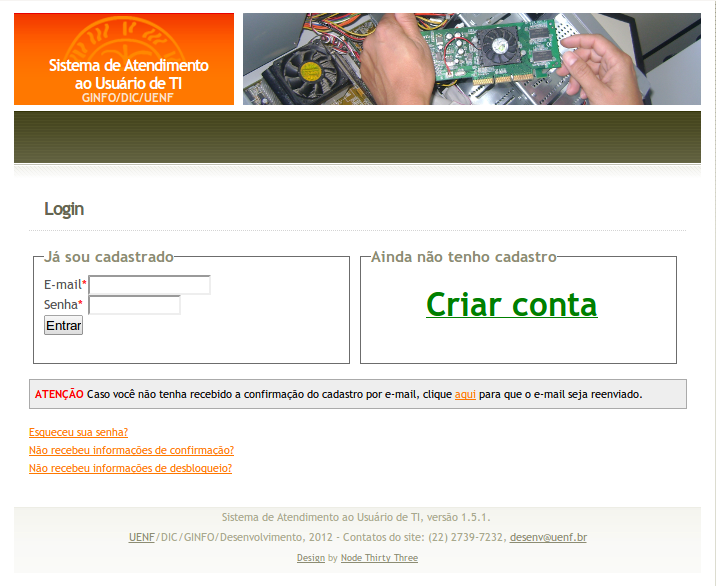
\includegraphics{figuras/login}}
    \caption{Tela de \textit{login} do sistema do setor}
\end{figure}

A Figura 6.1 apresenta a tela inicial do sistema. A tela deve ser carregada quando o endereço sistemas.uenf.br/suporte é acessado. Quanto o técnico inserir as informações de e-mail e senha, e clicar no botão ‘Entrar’, o sistema deverá carregar sua a página inicial, se o cadastro existir. Caso o técnico não tenha cadastro, o sistema deverá retornar uma mensagem avisando a não autenticação. Para ser criado um cadastro para um técnico é necessário comunicar com o responsável pelo desenvolvimento do sistema. Já para um solicitante, o cadastro é feito clicando no link ‘Criar conta’.

\newpage

\subsection{Tela 2 - Tela de dados pessoais}

\begin{figure}[ht]
    \centering
    \scalebox{0.6}{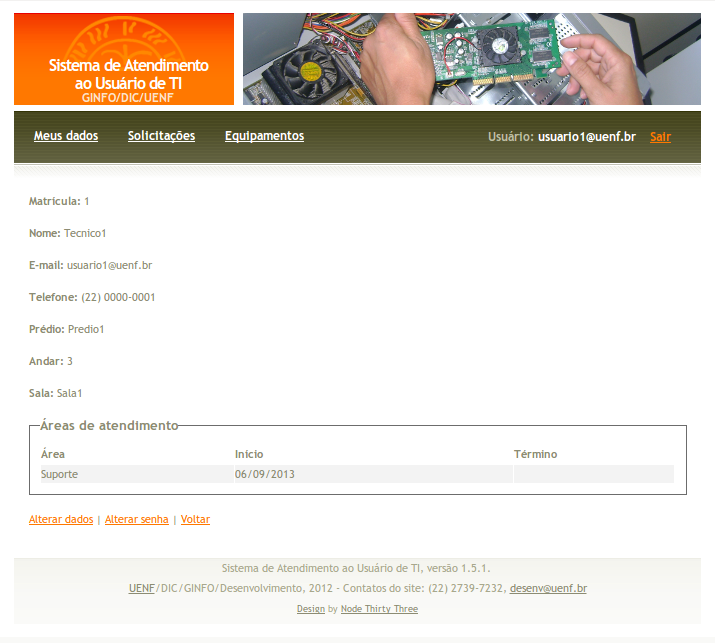
\includegraphics{figuras/home}}
    \caption{Tela inicial do técnico}
\end{figure}

A Figura 6.2 apresenta a tela inicial do técnico. Para carregá-la é preciso antes se autenticar no sistema através da tela representada na Figura 6.1. Nessa tela o técnico deverá poder visualizar e alterar seus dados pessoais bem como os referentes à sua área de atuação no setor. Quando alterada alguma informação e posteriormente enviadas para serem salvas, o sistema pode retornar erros de preenchimento segundo as críticas existentes, como por exemplo email inválido. 

\newpage

\subsection{Tela 3 - Tela das solicitações}

\begin{figure}[ht]
    \centering
    \scalebox{0.6}{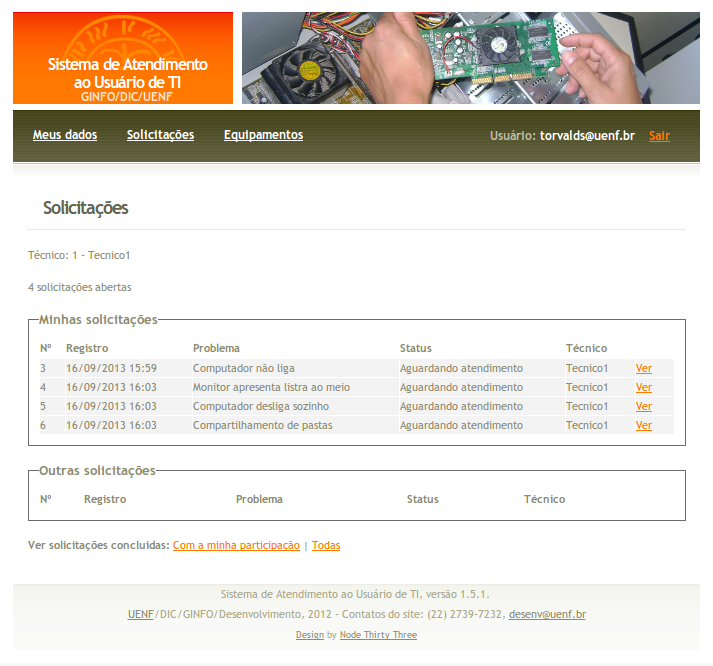
\includegraphics{figuras/solicitacoes}}
    \caption{Tela das solicitações}
\end{figure}

A Figura 6.3 representa a tela base das solicitações. Ela deverá ser carregada quando o técnico clicar no \textit{link} ‘Solicitações’ do menu de navegação, localizado na parte superior do sistema. A tela deverá apresentar, separadamente, todas as solicitações que estão sob a responsabilidade do técnico autenticado e as que estão sob a responsabilidade de outros técnicos. Ela também deverá permitir ao técnico visualizar as solicitações de forma específica. Ao clicar no \textit{link} ‘Ver’, presente na frente de cada solicitação, o sistema deverá carregar uma tela onde o técnico poderá checar todas as informações daquela solicitação. Nenhum erro pode ser gerado nessa tela.

\newpage

\subsection{Tela 4 - Tela de uma solicitação}

\begin{figure}[ht]
    \centering
    \scalebox{0.6}{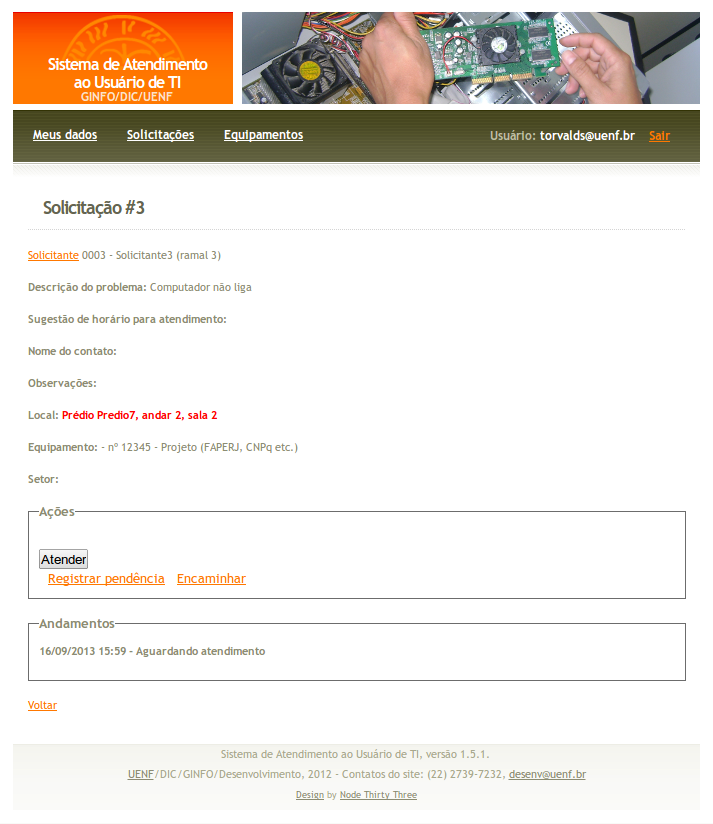
\includegraphics{figuras/solicitacao}}
    \caption{Tela de uma determinada solicitação}
\end{figure}

A Figura 6.4 apresenta a tela de uma determinada solicitação. Ela deverá ser carregada quando na tela representada pela Figura 6.3 o técnico clicar no \textit{link} ‘Ver’ presente na frente de cada solicitação. Esta tela deve fornecer ao técnico a possibilidade de execução de algumas ações em relação à solicitação, tais como ‘Atender’, ‘Registrar pendência’ ou ‘Encaminhar’. Ao clicar no \textit{link} ‘Atender’ deve surgir uma caixa de confirmação com a seguinte pergunta: ‘Esta solicitação entrará na fase de atendimento. Confirma?’; se o técnico clicar em ‘ok’, o sistema deverá carregar outras ações para a solicitação, como ‘Concluir’ e ‘Adicionar observação’.

\section{Execução do caso de uso}

O \textit{Raspberry Pi} foi utlizado segundo a tabela de dias e horários apresentada abaixo.

\begin{table}[!htpb]
 \centering
    \begin{tabular}{|p{2cm}|p{2cm}|p{2cm}|p{5cm}|p{2cm}|} 
    \hline
        \textbf{Dia} & \textbf{Usuário} & \textbf{Hora de início} & \textbf{Atividades realizadas} &  \textbf{Hora de término} \\
    \hline
         20/09/2013 & Técnico 1 & 15:33 & Técnico navegou pelas funcionalidades do sistema. & 15:45 \\
    \hline
        20/09/2013 & Técnico 2 & 15:57 & Além de navegar pelas funcionalidades do sistema, o técnico concluiu uma solicitação aberta. & 16:12 \\
    \hline
        20/09/2013 & Técnico 3 & 16:28 & Técnico navegou pelas funcionalidades do sistema. & 16:36 \\
    \hline
        20/09/2013 & Técnico 4 & 16:45 & Técnico navegou pelas funcionalidades do sistema e checou caixa de emails. & 17:03 \\
    \hline
        02/10/2013 & Técnico 5 & 12:33 & Técnico navegou pelas funcionalidades do sistema. & 12:46 \\
    \hline
    \end{tabular}
    \caption{Informações dos testes realizados pelos técnicos do setor}
    \label{t_fixa}
\end{table}

Durante a avaliação realizada pelos usuários não ocorreram falhas.

\section{Questionário}

O questionário tem como objetivo capturar o \textit{momento da verdade} de uso do dispositivo e apoiar a avaliação de sua adequação sob o ponto de vista dos usuários.

Abaixo de cada pergunta existiam cinco opções de resposta enumeradas de 1 a 5, e um texto de ajuda com a seguinte frase: “Assinale uma resposta entre 1 e 5, sendo 1 para a pior qualificação possível ou 5 para a melhor.”.
As perguntas foram apresentadas dessa forma:

\textbf{P1.} O hardware \textit{Raspberry Pi} é fácil de ser colocado em funcionamento?

\textbf{P2.} Você achou confortável o desempenho do equipamento ao executar o navegador (\textit{browser}) para acessar o site do sistema?

\textbf{P3.} Ao navegar pelo sistema e executar algumas de suas funcionalidades o desempenho do equipamento foi satisfatório?

\textbf{P4.} Como você avalia o equipamento com relação a travamentos quando executada alguma funcionalidade do sistema?

\textbf{P5.} Como você avalia o equipamento com relação a travamentos ocorridos em qualquer momento, seja utilizando as funcionalidades do sistema ou não?

\textbf{P6.} Levando em consideração somente a execução das funcionalidades pertinentes ao seu ambiente de produção, o quanto você acha viável a substituição de sua estação de trabalho por este equipamento avaliado?

\textbf{P7.} Dado que você precise de um computador para manipular um sistema semelhante ao do setor avaliado, o quanto você acha viável a utilização do equipamento apresentado?

\textbf{P8.} Levando em consideração a existência de um negócio seu que ainda não é informatizado, e sabendo que o preço de um \textit{Raspberry Pi} é  R\$ 176,02, o quanto o custo do equipamento apoia a ideia da criação de um sistema informatizado para gerenciar sua empresa?

\textbf{P9.} De um forma geral, você aprovou o equipamento avaliado?
 % Cria o capítulo 6
\chapter{RESULTADOS OBTIDOS}

O \textit{Raspberry Pi} não é rápido o suficiente para realizar trabalhos que façam uso intensivo de leitura e escrita, como um servidor por exemplo. Entretanto é suficientemente rápido para aplicações standalone, quando não há um uso excessivo dos recursos do equipamento.

Seu custo é razoável para aquisição de uma primeira máquina, mas sua compra em larga escala não é viável por dificuldade de fornecimento e pela dificuldade de suporte local.

Sua utilização como estação de trabalho para ambiente web é suficientemente estável, mas ao acessar sites que demandam um uso mais intenso de memória, a navegação se torna desconfortável e demorada.

Durante o estudo de caso as funcionalidades foram testadas com sucesso, sem a ocorrência de qualquer falha, gerando nas pessoas que utilizaram o sistema uma impressão aparentemente positiva em relação ao equipamento apresentado. As respostas são apresentadas na tabela 7.1.

\begin{table}[!htpb]
 \centering
    \begin{tabular}{|c|c|c|c|c|c|c|c|c|c|} 
    \hline
        \textbf{Usuário} & \textbf{P1} & \textbf{P2} & \textbf{P3} & \textbf{P4} & \textbf{P5} & \textbf{P6} & \textbf{P7} & \textbf{P8} & \textbf{P9} \\
    \hline
        Técnico 1 & 5 & 4 & 5 & 5 & 5 & 3 & 3 & 4 & 4 \\
    \hline
        Técnico 2 & 5 & 5 & 4 & 4 & 4 & 5 & 5 & 5 & 5 \\
    \hline
        Técnico 3  & 5 & 4 &	4 &	5 &	5 &	5 &	5 &	4 &	4 \\
    \hline
    	Técnico 4  & 5 & 5 &	5 &	5 &	5 &	5 &	5 &	5 &	5 \\
    \hline
 	    Técnico 5  & 5 & 5 & 5 & 5 & 5 & 4 & 5 & 4 & 5 \\
    \hline
    \end{tabular}
    \caption{Respostas dos técnicos obtidas através do questionário}
    \label{t_fixa}
\end{table}

A primeira pergunta tinha como objetivo avaliar o nível de facilidade para colocar o \textit{Raspberry Pi} em funcionamento. A segunda e a terceira eram relacionadas ao desempenho do \textit{browser} para acessar o site da aplicação e para manipulá-lo. A quarta e a quinta capturaram do usuário se o equipamento travou quando executada algumas funcionalidades do sistema ou em qualquer outro momento.

A sexta tinha como objetivo quantificar a ideia de trocar o desktop do usuário pelo \textit{Raspberry Pi}. A sétima quantificava o uso do Pi em qualquer outro negócio que tivesse um sistema semelhante ao do setor. A oitava perguntava ao usuário se o preço do equipamento reforçava a construção de um sistema web para sua empresa, caso fosse dono de uma. E a nona concluía o questionário perguntando ao usuário se ele aprovava o equipamento de uma forma geral.

O \textit{Raspberry Pi} obteve uma aprovação total de aproximadamente 93\% dos usuários. Tal resultado corrobora com a opinião de que a experiência pode ser positiva para pequenas empresas. % Cria o capítulo 7
\chapter{CONCLUSÃO}

\section{Objetivos alcançados}

Após todo o procedimento de testes de implantação e uso do hardware Raspberry Pi no ambiente de produção do estudo de caso, e posterior análise dos questionários preenchidos pelos usuários convidados para realizar o uso do equipamento, conclui-se que ele é uma boa alternativa em pequenas empresas.
Os custos discutidos deixam claro que o equipamento é uma oportunidade de diminuir o gasto para se montar sistemas computacionais, pois, como ficou evidenciado neste trabalho, o preço de um Raspberry Pi é, aproximadamente, 39\% menor que um computador desktop.

As configurações apresentadas demonstram que o equipamento é suficientemente flexível para atender a diversas necessidades comuns, bem como inovadoras.
A pergunta 9, considerada importante para este estudo de caso obteve uma resposta positiva de 100\% dos respondentes, corroborando com as hipóteses de vantagem no uso do equipamento. Sendo assim, nota-se que a totalidade dos usuários aprovou o uso do Raspberry Pi no seu ambiente de produção.

Conclui-se, portanto, que a tecnologia apresentada neste trabalho foi considerada perfeitamente capaz de ser utilizada como meio de manipulação do sistema informatizado do setor, permitindo formar expectativas em relação à possibilidade de que o equipamento apresentado possa atingir uma visibilidade e usabilidade maiores em pequenas empresas, visto que muitas dessas organizações deixam de informatizar o seu negócio por causa dos elevados custos de compra e manutenção de computadores.

\section{Trabalhos Futuros}

Este trabalho mostrou que o Raspberry Pi obteve um bom desempenho quando utilizado para acessar e manipular sistemas desenvolvidos para a web, entretando sabe-se que existem sistemas desktop e que eles utilizam os recursos do equipamento onde fica hospedado. Sendo assim, seria interessante conhecer os limites impostos pelo Raspberry Pi quanto à instalação e utilização de sistemas com tais características. % Cria o capítulo 8
\bibliography{referencia} % Gera as referências bibliográficas
\appendix

\chapter{Comparativo de preços}

\begin{table}[!htpb]
 \centering
    \begin{tabular}{|p{4cm}|p{2cm}|p{4cm}|p{4cm}|} 
    \hline
        \textbf{Periféricos} & \textbf{Preço} & \textbf{Sistema Computacional com \textit{Raspberry Pi}} & \textbf{Sistema Computacional com \textit{desktop}} \\
    \hline
        Monitor c/ entrada HDMI & R\$ 404,10 & X & X \\
    \hline
        Cabo HDMI & R\$ 14,90 & X & X \\
    \hline
        Mouse USB & R\$ 9,99 & X & \\
    \hline
        Teclado USB & R\$ 22,40 & X & \\
    \hline
        Cartão MicroSD 8GB com adaptador & R\$ 32,52 & X & \\
    \hline
        Carregador Micro USB (fonte de alimentação) & R\$ 39,90 & X & \\
    \hline
        Cabo de força (fonte de alimentação) & R\$ 5,30 & & X \\
    \hline
        Placa \textit{Raspberry Pi} & R\$ 176,02 & X & \\
    \hline
        \textit{Desktop} (mouse e teclado inclusos) & R\$ 719,10 & & X \\
    \hline
        \textbf{TOTAL} & & \textbf{R\$ 699,83} & \textbf{R\$ 1.143,40} \\
    \hline
    \end{tabular}
    \caption{Comparativo entre sistemas computacionais}
    \label{t_fixa}
\end{table}

\chapter{Questionário}

\begin{figure}[ht]
    \centering
    \scalebox{0.4}{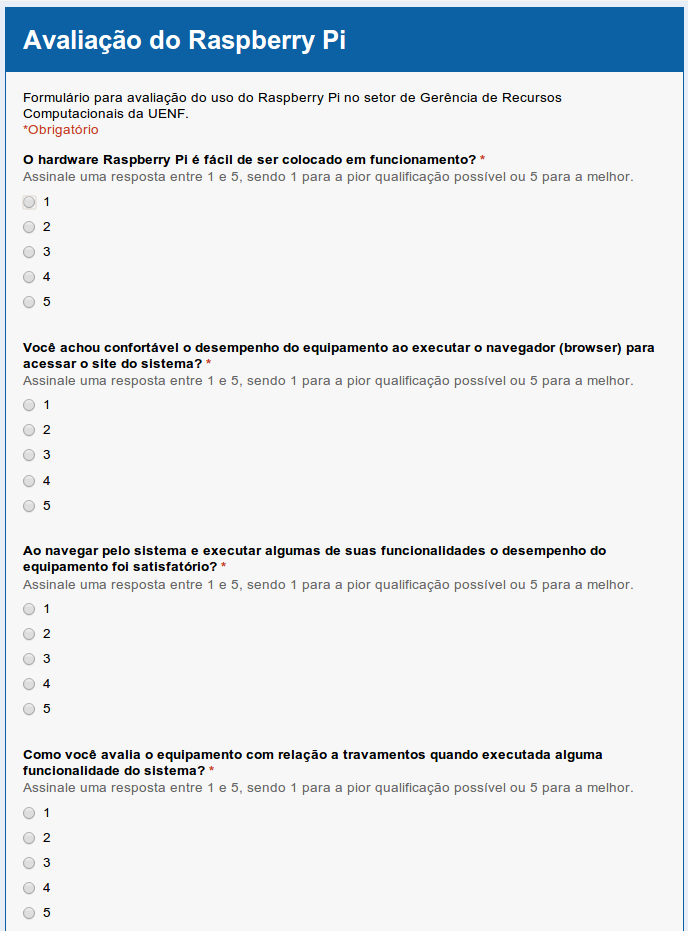
\includegraphics{figuras/questionario1}}
    \caption{Primeira parte do questionário}
\end{figure}

\begin{figure}[ht]
    \centering
    \scalebox{0.4}{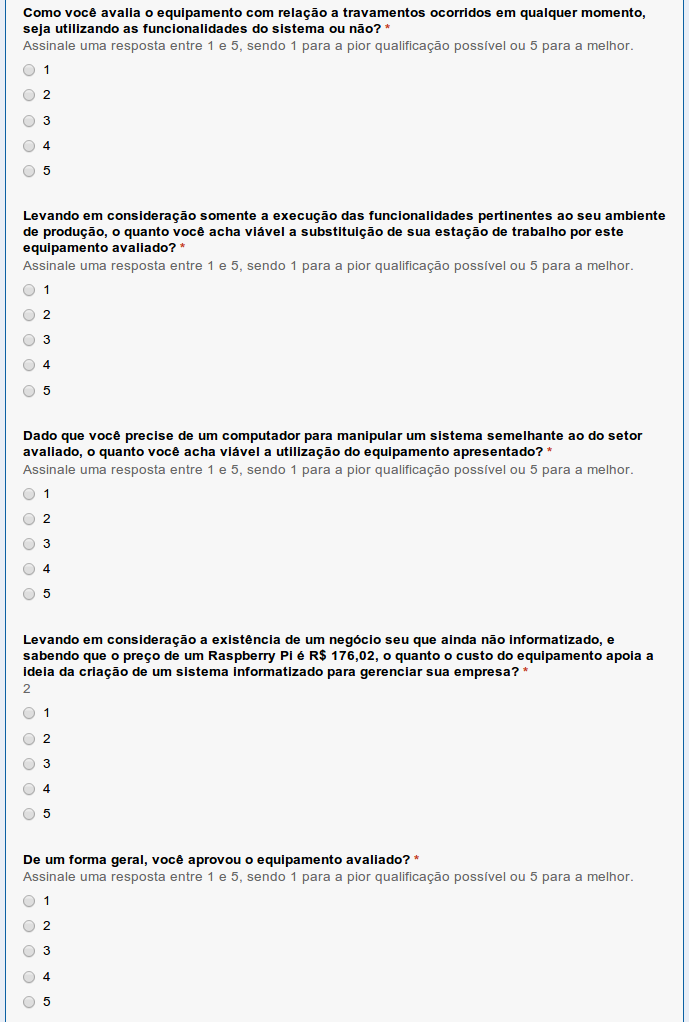
\includegraphics{figuras/questionario2}}
    \caption{Segunda parte do questionário}
\end{figure} % Cria o apêndice
\end{document} % Fim do TCC
